\lhead{\emph{Identifier Arrays}}
\chapter{Identifier Arrays}

The easiest and probably most intuitive way of dealing with classification task is to use patterns' spatial relations in order to determine their class memberships. This approach is used for example in kNN and SVM models, where point's affiliation is calculated based on its place in the features space. Every class in a dataset can be viewed as a big ``cloud`` of points and usually, if the other clouds do not overlap each other, the more dense this cloud is, the easier the task of classification gets.

Each class' cloud can be enclosed in an arbitrary geometrical shape which can be used as an identifier. The difference between binary classifiers and identifiers is very subtle, yet important. Whereas binary classifiers can distinguish between patterns from two different classes, they must be trained on data consisting of elements from both classes. Identifiers accept (or one could say: identify) only those points that they were constructed on, and reject any outliers. Thus they require only one class to be provided during training process. One of the easiest and most intuitive model of identifier is minimum volume enclosing figure. Creating figure enclosing all elements that has the smallest volume possible ensures that the identification can be very strict, which in return helps to maintain high outlier rejection rate. As opposed to convex hull, which is the most accurate point set container with smallest volume and which is enclosed by linear hyperplanes, bounding figures are far less complex. In many cases, when there is a need for computing convex hull and testing inclusions of other points, an approximation of such hull can be used, which helps in reducing time needed for computations, since most of alternative methods have lower construction and inclusion-testing complexities. Among the most popular minimum volume enclosing figures there are: boxes, diamonds, simplexes and ellipsoids.

\section{Minimum Volume Enclosing Ellipsoid}

Minimum Volume Enclosing Ellipsoid (denoted as MVEE) problem is solved by several known algorithms that can be categorized as first-order, second-order interior-point or combination of the two. For small dimensions \textit{d}, the MVEE problem can be solved in \textit{O($d^{O(d)}$m)} operations using randomized or deterministic algorithms~\cite{MVEEMichaelTodd2005}. All the results presented in this chapter were obtained while using MVEE algorithm based on Khachiyan solution.

An ellipsoid in its centre form is given by the formula:
\vspace{-6pt} 
\[ 
\vspace{-3pt}
E = \{x \in \mathbb{R}^{n} | (x - c)^{T}A(x-c) \le 1\} 
\vspace{-3pt}
\] 
where $c \in \mathbb{R}^{n}$ is the centre of the ellipse E and $ A \in \mathbb{S}^{n}_{++}$ is a positive definite matrix. Points lying inside the ellipsoid satisfy 
\begin{equation}\label{eq:ellipsoid_affiliation}(x_{i} - c)^{T}A(x_{i} - c) \le 1 + \varepsilon\end{equation}
where $\varepsilon$ parameter defines the error margin in determining whether certain point belongs to ellipsoid. It can also be used ``enlarge`` the ellipsoid (by increasing $\varepsilon$ value).% It can be imagined as testing point inclusion on enlarged ellipsoid.

However, constructing minimal volume bounding ellipsoid is not a convex optimization problem. It turns out that the solution is not easily obtainable so the dual problem has to be found. For a more precise and in depth solution description see \cite{MVEEMichaelTodd2005}. The main problem, when using ellipsoids as identifiers, lies in constructing them. Two main factors that decide about identification effectiveness are tolerance and acceptance parameters. Tolerance can be viewed as a threshold for ellipsoid construction accuracy. The lower the parameter is, the better minimal volume ellipsoid is created. On the other hand, even with a good training set, there is a risk of including native patterns that lie outside of the created ellipsoid. Acceptance parameter has been introduced to prevent such unwanted behaviour. It defines a threshold for point rejection for elements lying outside of the created figure.

\section{Ellipsoids array classifier}

The construction of a classifier using array of identifiers is pretty simple and straightforward. The array is filled with ellipsoids, one for each class in the training dataset. Every unknown pattern, sent for classification, moves through those ellipsoids and gets the information whether it lies inside the ellipsoid or not. In case of being part of identifier's interior the value given by the equation (\ref{eq:ellipsoid_affiliation}) is taken into consideration, which tells about the position inside the ellipsoid (where value 0 means that the point is in the ellipsoid's centre and 1 means that it lies on the surface). Finally, after all ellipsoids are checked, the one with the smallest equation (\ref{eq:ellipsoid_affiliation}) value (and for which the point lies inside it), designates the class to which this unknown pattern should be classified to. If no ellipsoid accepts the point, it is rejected and treated as a foreign element. 

One way of increasing rejection ratio would be to decrease ellipsoid size. The smaller the volume the less points lie inside, which in turn boosts rejection rates but worsens classification. Changing ellipsoid size can be helpful in a situation in which two classes overlap and rejection of the elements is more desired result than misclassification.

\begin{figure}[htp]
	\centering
	
\includegraphics[width=0.8\textwidth]{Figures/ellipsoids_array_example.png}
	\caption{ Array of ellipsoids that works as a classifier with rejection capabilities. Elements outside of existing ellipsoids are treated as a foreign patterns. }
	\label{fig:ellipsoids_array}\vspace{-3pt}
\end{figure}


\section{Results}

The tests were performed and their results were stored in the same manner as in similar tests in previous chapters. The classification and rejection rates for identifier array using ellipsoids are very good, staying within 85\% - 95\% value.

\begin{table}[htp]
	\centering
	\caption{Results obtained for Ellipsoid arrays}
	\label{ellipsoid_arrays_results}
	\begin{tabular}{l|c|lll}
		\cline{2-2}
		& \multicolumn{1}{l|}{\textbf{Ellipsoid}} &  &  &  \\ \cline{1-2}
		\multicolumn{1}{|l|}{\textbf{Strict Accuracy}}           & 88.28 \\ \cline{1-2}
		\multicolumn{1}{|l|}{\textbf{Fine Accuracy}}             & 93.14 \\ \cline{1-2}
		\multicolumn{1}{|l|}{\textbf{Strict Native Sensitivity}} & 83.95 \\ \cline{1-2}
		\multicolumn{1}{|l|}{\textbf{Accuracy}}                  & 89.98 \\ \cline{1-2}
		\multicolumn{1}{|l|}{\textbf{Native Precision}}          & 77.23 \\ \cline{1-2}
		\multicolumn{1}{|l|}{\textbf{Native Sensitivity}}        & 90.13 \\ \cline{1-2}
		\multicolumn{1}{|l|}{\textbf{Native F-measure}}          & 83.18 \\ \cline{1-2}
		\multicolumn{1}{|l|}{\textbf{Foreign Precision}}         & 96.01 \\ \cline{1-2}
		\multicolumn{1}{|l|}{\textbf{Foreign Sensitivity}}       & 89.93 \\ \cline{1-2}
		\multicolumn{1}{|l|}{\textbf{Foreign F-measure}}         & 92.87 \\ \cline{1-2}
	\end{tabular}
\end{table}

Although it may seem that the ellipsoids are superior to other classifiers presented and used in this paper it is worth noting that the tests were performed on only one dataset. Geometric classifiers that work on raw data, without introducing any changes to feature values given during training don't work well in situations when class elements overlap. SVM, random forest, etc. which should be used in such cases have the advantage over simple classifiers like kNN or arrays of minimum volume enclosing figures, because they change the way features are interpreted. For example, SVM increases dimensionality by using kernel function to introduce such feature-space representation in which two different classes are easily separated by a hyperplane.

\section{Optimizing ellipsoid size}

One thing worth noting when using ellipsoids is that their size can be easily enlarged when having few points that are located far away from their class centre. This situation can lead to decrease in rejection option rates as well as bigger misclassification between native elements' classes. Of course decreasing ellipsoid size can result in the opposite situation. The key to deal with this difficulty is to find balance between decreasing ellipsoid size and still getting high rejection and classification rates. Two approaches are proposed in this paper.

\subsection{Tolerance parameter manipulation}

The tolerance parameter, also named as $\varepsilon$ in Equation (\ref{eq:ellipsoid_affiliation}), can be used during point affiliation check-up to manipulate the result of the equation. By decreasing its value the ellipsoid ``shrinks`` evenly in all directions, and by increasing it more points are accepted as if they were lying inside the ellipsoid. Overall 10 tests there were performed with $\varepsilon$ consecutive values being~$(2^{0}, 2^{-1}, 2^{-2}, \dots, 2^{-10})$. The results can be seen in Figure \ref{fig:shrinking_ellipsoids_tolerance_manipulation}

\begin{figure}[htp]
	\centering
	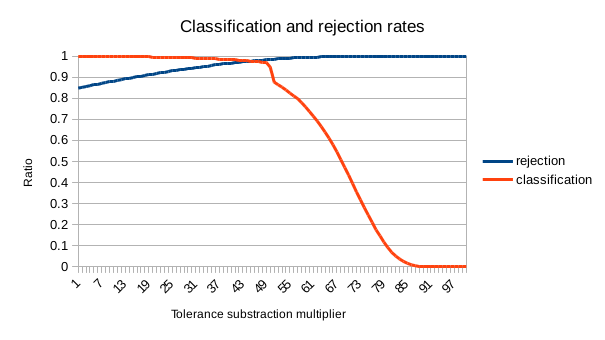
\includegraphics[width=0.8\textwidth]{Figures/shrinking_ellipsoid_tolerance_manipulation.png}
	\caption{ Classification and rejection rates for different $\varepsilon$ value  }
	\label{fig:shrinking_ellipsoids_tolerance_manipulation}\vspace{-3pt}
\end{figure}

\subsection{Native elements rejection}

The problem with manipulating the tolerance parameter is that ...
Another approach towards shrinking ellipsoids

\begin{figure}[htp]
	\centering
	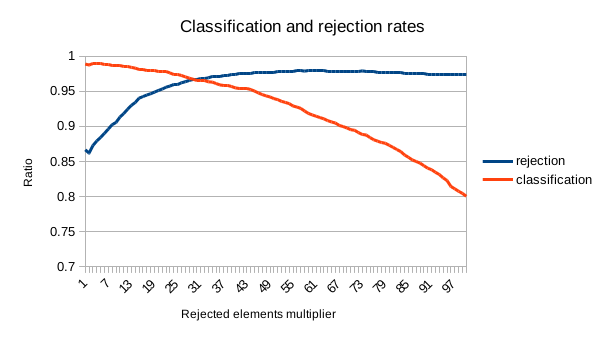
\includegraphics[width=0.8\textwidth]{Figures/shrinking_ellipsoid_elements_rejection.png}
	\caption{  }
	\label{fig:shrinking_ellipsoids_elements_rejection}\vspace{-3pt}
\end{figure}

\section{Summary}

The tests performed on the classifier using array of identifiers prove that it can successfully combine classification and rejection tasks. While being unable to do the multi-class classification on their own, combined ellipsoids can be very accurate at classification and rejecting foreigners. Minimum volume enclosing ellipsoids combine advantages of commonly used classifiers described in Chapter \ref{common_classifiers} such as easy point inclusion detection, and iterative construction algorithm that uses tolerance parameter for its stop condition. The main disadvantage of ellipsoid, and minimum volume enclosing figures in general, is the fact that it does not transform the feature space of presented data. In order to get good results the data should be separable, and no generalisation of information is done at all. This is completely different from the attitude introduced in random forest or svm.
